
%% bare_jrnl.tex
%% V1.3
%% 2007/01/11
%% by Michael Shell
%% see http://www.michaelshell.org/
%% for current contact information.
%%
%% This is a skeleton file demonstrating the use of IEEEtran.cls
%% (requires IEEEtran.cls version 1.7 or later) with an IEEE journal paper.
%%
%% Support sites:
%% http://www.michaelshell.org/tex/ieeetran/
%% http://www.ctan.org/tex-archive/macros/latex/contrib/IEEEtran/
%% and
%% http://www.ieee.org/



% *** Authors should verify (and, if needed, correct) their LaTeX system  ***
% *** with the testflow diagnostic prior to trusting their LaTeX platform ***
% *** with production work. IEEE's font choices can trigger bugs that do  ***
% *** not appear when using other class files.                            ***
% The testflow support page is at:
% http://www.michaelshell.org/tex/testflow/


%%*************************************************************************
%% Legal Notice:
%% This code is offered as-is without any warranty either expressed or
%% implied; without even the implied warranty of MERCHANTABILITY or
%% FITNESS FOR A PARTICULAR PURPOSE! 
%% User assumes all risk.
%% In no event shall IEEE or any contributor to this code be liable for
%% any damages or losses, including, but not limited to, incidental,
%% consequential, or any other damages, resulting from the use or misuse
%% of any information contained here.
%%
%% All comments are the opinions of their respective authors and are not
%% necessarily endorsed by the IEEE.
%%
%% This work is distributed under the LaTeX Project Public License (LPPL)
%% ( http://www.latex-project.org/ ) version 1.3, and may be freely used,
%% distributed and modified. A copy of the LPPL, version 1.3, is included
%% in the base LaTeX documentation of all distributions of LaTeX released
%% 2003/12/01 or later.
%% Retain all contribution notices and credits.
%% ** Modified files should be clearly indicated as such, including  **
%% ** renaming them and changing author support contact information. **
%%
%% File list of work: IEEEtran.cls, IEEEtran_HOWTO.pdf, bare_adv.tex,
%%                    bare_conf.tex, bare_jrnl.tex, bare_jrnl_compsoc.tex
%%*************************************************************************

% Note that the a4paper option is mainly intended so that authors in
% countries using A4 can easily print to A4 and see how their papers will
% look in print - the typesetting of the document will not typically be
% affected with changes in paper size (but the bottom and side margins will).
% Use the testflow package mentioned above to verify correct handling of
% both paper sizes by the user's LaTeX system.
%
% Also note that the "draftcls" or "draftclsnofoot", not "draft", option
% should be used if it is desired that the figures are to be displayed in
% draft mode.
%
\documentclass[draftclsnofoot,12pt,journal,onecolumn]{IEEEtran}
\renewcommand{\rmdefault}{phv} % Arial
\renewcommand{\sfdefault}{phv} % Arial
\setcounter{page}{3}

%
% If IEEEtran.cls has not been installed into the LaTeX system files,
% manually specify the path to it like:
% \documentclass[journal]{../sty/IEEEtran}





% Some very useful LaTeX packages include:
% (uncomment the ones you want to load)


% *** MISC UTILITY PACKAGES ***
%
\usepackage{ifpdf}
% Heiko Oberdiek's ifpdf.sty is very useful if you need conditional
% compilation based on whether the output is pdf or dvi.
% usage:
% \ifpdf
%   % pdf code
% \else
%   % dvi code
% \fi
% The latest version of ifpdf.sty can be obtained from:
% http://www.ctan.org/tex-archive/macros/latex/contrib/oberdiek/
% Also, note that IEEEtran.cls V1.7 and later provides a builtin
% \ifCLASSINFOpdf conditional that works the same way.
% When switching from latex to pdflatex and vice-versa, the compiler may
% have to be run twice to clear warning/error messages.






% *** CITATION PACKAGES ***
%
\usepackage{cite}
% cite.sty was written by Donald Arseneau
% V1.6 and later of IEEEtran pre-defines the format of the cite.sty package
% \cite{} output to follow that of IEEE. Loading the cite package will
% result in citation numbers being automatically sorted and properly
% "compressed/ranged". e.g., [1], [9], [2], [7], [5], [6] without using
% cite.sty will become [1], [2], [5]--[7], [9] using cite.sty. cite.sty's
% \cite will automatically add leading space, if needed. Use cite.sty's
% noadjust option (cite.sty V3.8 and later) if you want to turn this off.
% cite.sty is already installed on most LaTeX systems. Be sure and use
% version 4.0 (2003-05-27) and later if using hyperref.sty. cite.sty does
% not currently provide for hyperlinked citations.
% The latest version can be obtained at:
% http://www.ctan.org/tex-archive/macros/latex/contrib/cite/
% The documentation is contained in the cite.sty file itself.



%\usepackage{hyperref}


% *** GRAPHICS RELATED PACKAGES ***
%
\ifCLASSINFOpdf
  % \usepackage[pdftex]{graphicx}
  % declare the path(s) where your graphic files are
  % \graphicspath{{../pdf/}{../jpeg/}}
  % and their extensions so you won't have to specify these with
  % every instance of \includegraphics
  % \DeclareGraphicsExtensions{.pdf,.jpeg,.png}
\else
  % or other class option (dvipsone, dvipdf, if not using dvips). graphicx
  % will default to the driver specified in the system graphics.cfg if no
  % driver is specified.
   \usepackage[dvips]{graphicx}
  % declare the path(s) where your graphic files are
   \graphicspath{{./figures/}}
  % and their extensions so you won't have to specify these with
  % every instance of \includegraphics
  % \DeclareGraphicsExtensions{.eps}
\fi
% graphicx was written by David Carlisle and Sebastian Rahtz. It is
% required if you want graphics, photos, etc. graphicx.sty is already
% installed on most LaTeX systems. The latest version and documentation can
% be obtained at: 
% http://www.ctan.org/tex-archive/macros/latex/required/graphics/
% Another good source of documentation is "Using Imported Graphics in
% LaTeX2e" by Keith Reckdahl which can be found as epslatex.ps or
% epslatex.pdf at: http://www.ctan.org/tex-archive/info/
%
% latex, and pdflatex in dvi mode, support graphics in encapsulated
% postscript (.eps) format. pdflatex in pdf mode supports graphics
% in .pdf, .jpeg, .png and .mps (metapost) formats. Users should ensure
% that all non-photo figures use a vector format (.eps, .pdf, .mps) and
% not a bitmapped formats (.jpeg, .png). IEEE frowns on bitmapped formats
% which can result in "jaggedy"/blurry rendering of lines and letters as
% well as large increases in file sizes.
%
% You can find documentation about the pdfTeX application at:
% http://www.tug.org/applications/pdftex





% *** MATH PACKAGES ***
%
\usepackage[cmex10]{amsmath}
\usepackage{amsfonts}
% A popular package from the American Mathematical Society that provides
% many useful and powerful commands for dealing with mathematics. If using
% it, be sure to load this package with the cmex10 option to ensure that
% only type 1 fonts will utilized at all point sizes. Without this option,
% it is possible that some math symbols, particularly those within
% footnotes, will be rendered in bitmap form which will result in a
% document that can not be IEEE Xplore compliant!
%
% Also, note that the amsmath package sets \interdisplaylinepenalty to 10000
% thus preventing page breaks from occurring within multiline equations. Use:
%\interdisplaylinepenalty=2500
% after loading amsmath to restore such page breaks as IEEEtran.cls normally
% does. amsmath.sty is already installed on most LaTeX systems. The latest
% version and documentation can be obtained at:
% http://www.ctan.org/tex-archive/macros/latex/required/amslatex/math/





% *** SPECIALIZED LIST PACKAGES ***
%
%\usepackage{algorithmic}
% algorithmic.sty was written by Peter Williams and Rogerio Brito.
% This package provides an algorithmic environment fo describing algorithms.
% You can use the algorithmic environment in-text or within a figure
% environment to provide for a floating algorithm. Do NOT use the algorithm
% floating environment provided by algorithm.sty (by the same authors) or
% algorithm2e.sty (by Christophe Fiorio) as IEEE does not use dedicated
% algorithm float types and packages that provide these will not provide
% correct IEEE style captions. The latest version and documentation of
% algorithmic.sty can be obtained at:
% http://www.ctan.org/tex-archive/macros/latex/contrib/algorithms/
% There is also a support site at:
% http://algorithms.berlios.de/index.html
% Also of interest may be the (relatively newer and more customizable)
% algorithmicx.sty package by Szasz Janos:
% http://www.ctan.org/tex-archive/macros/latex/contrib/algorithmicx/




% *** ALIGNMENT PACKAGES ***
%
%\usepackage{array}
% Frank Mittelbach's and David Carlisle's array.sty patches and improves
% the standard LaTeX2e array and tabular environments to provide better
% appearance and additional user controls. As the default LaTeX2e table
% generation code is lacking to the point of almost being broken with
% respect to the quality of the end results, all users are strongly
% advised to use an enhanced (at the very least that provided by array.sty)
% set of table tools. array.sty is already installed on most systems. The
% latest version and documentation can be obtained at:
% http://www.ctan.org/tex-archive/macros/latex/required/tools/


%\usepackage{mdwmath}
%\usepackage{mdwtab}
% Also highly recommended is Mark Wooding's extremely powerful MDW tools,
% especially mdwmath.sty and mdwtab.sty which are used to format equations
% and tables, respectively. The MDWtools set is already installed on most
% LaTeX systems. The lastest version and documentation is available at:
% http://www.ctan.org/tex-archive/macros/latex/contrib/mdwtools/


% IEEEtran contains the IEEEeqnarray family of commands that can be used to
% generate multiline equations as well as matrices, tables, etc., of high
% quality.


%\usepackage{eqparbox}
% Also of notable interest is Scott Pakin's eqparbox package for creating
% (automatically sized) equal width boxes - aka "natural width parboxes".
% Available at:
% http://www.ctan.org/tex-archive/macros/latex/contrib/eqparbox/





% *** SUBFIGURE PACKAGES ***
\usepackage[tight,footnotesize]{subfigure}
% subfigure.sty was written by Steven Douglas Cochran. This package makes it
% easy to put subfigures in your figures. e.g., "Figure 1a and 1b". For IEEE
% work, it is a good idea to load it with the tight package option to reduce
% the amount of white space around the subfigures. subfigure.sty is already
% installed on most LaTeX systems. The latest version and documentation can
% be obtained at:
% http://www.ctan.org/tex-archive/obsolete/macros/latex/contrib/subfigure/
% subfigure.sty has been superceeded by subfig.sty.



%\usepackage[caption=false]{caption}
%\usepackage[font=footnotesize,caption=false]{subfig}
% subfig.sty, also written by Steven Douglas Cochran, is the modern
% replacement for subfigure.sty. However, subfig.sty requires and
% automatically loads Axel Sommerfeldt's caption.sty which will override
% IEEEtran.cls handling of captions and this will result in nonIEEE style
% figure/table captions. To prevent this problem, be sure and preload
% caption.sty with its "caption=false" package option. This is will preserve
% IEEEtran.cls handing of captions. Version 1.3 (2005/06/28) and later 
% (recommended due to many improvements over 1.2) of subfig.sty supports
% the caption=false option directly:
%\usepackage[caption=false,font=footnotesize]{subfig}
%
% The latest version and documentation can be obtained at:
% http://www.ctan.org/tex-archive/macros/latex/contrib/subfig/
% The latest version and documentation of caption.sty can be obtained at:
% http://www.ctan.org/tex-archive/macros/latex/contrib/caption/




% *** FLOAT PACKAGES ***
%
%\usepackage{fixltx2e}
% fixltx2e, the successor to the earlier fix2col.sty, was written by
% Frank Mittelbach and David Carlisle. This package corrects a few problems
% in the LaTeX2e kernel, the most notable of which is that in current
% LaTeX2e releases, the ordering of single and double column floats is not
% guaranteed to be preserved. Thus, an unpatched LaTeX2e can allow a
% single column figure to be placed prior to an earlier double column
% figure. The latest version and documentation can be found at:
% http://www.ctan.org/tex-archive/macros/latex/base/



%\usepackage{stfloats}
% stfloats.sty was written by Sigitas Tolusis. This package gives LaTeX2e
% the ability to do double column floats at the bottom of the page as well
% as the top. (e.g., "\begin{figure*}[!b]" is not normally possible in
% LaTeX2e). It also provides a command:
%\fnbelowfloat
% to enable the placement of footnotes below bottom floats (the standard
% LaTeX2e kernel puts them above bottom floats). This is an invasive package
% which rewrites many portions of the LaTeX2e float routines. It may not work
% with other packages that modify the LaTeX2e float routines. The latest
% version and documentation can be obtained at:
% http://www.ctan.org/tex-archive/macros/latex/contrib/sttools/
% Documentation is contained in the stfloats.sty comments as well as in the
% presfull.pdf file. Do not use the stfloats baselinefloat ability as IEEE
% does not allow \baselineskip to stretch. Authors submitting work to the
% IEEE should note that IEEE rarely uses double column equations and
% that authors should try to avoid such use. Do not be tempted to use the
% cuted.sty or midfloat.sty packages (also by Sigitas Tolusis) as IEEE does
% not format its papers in such ways.


%\ifCLASSOPTIONcaptionsoff
%  \usepackage[nomarkers]{endfloat}
% \let\MYoriglatexcaption\caption
% \renewcommand{\caption}[2][\relax]{\MYoriglatexcaption[#2]{#2}}
%\fi
% endfloat.sty was written by James Darrell McCauley and Jeff Goldberg.
% This package may be useful when used in conjunction with IEEEtran.cls'
% captionsoff option. Some IEEE journals/societies require that submissions
% have lists of figures/tables at the end of the paper and that
% figures/tables without any captions are placed on a page by themselves at
% the end of the document. If needed, the draftcls IEEEtran class option or
% \CLASSINPUTbaselinestretch interface can be used to increase the line
% spacing as well. Be sure and use the nomarkers option of endfloat to
% prevent endfloat from "marking" where the figures would have been placed
% in the text. The two hack lines of code above are a slight modification of
% that suggested by in the endfloat docs (section 8.3.1) to ensure that
% the full captions always appear in the list of figures/tables - even if
% the user used the short optional argument of \caption[]{}.
% IEEE papers do not typically make use of \caption[]'s optional argument,
% so this should not be an issue. A similar trick can be used to disable
% captions of packages such as subfig.sty that lack options to turn off
% the subcaptions:
% For subfig.sty:
% \let\MYorigsubfloat\subfloat
% \renewcommand{\subfloat}[2][\relax]{\MYorigsubfloat[]{#2}}
% For subfigure.sty:
% \let\MYorigsubfigure\subfigure
% \renewcommand{\subfigure}[2][\relax]{\MYorigsubfigure[]{#2}}
% However, the above trick will not work if both optional arguments of
% the \subfloat/subfig command are used. Furthermore, there needs to be a
% description of each subfigure *somewhere* and endfloat does not add
% subfigure captions to its list of figures. Thus, the best approach is to
% avoid the use of subfigure captions (many IEEE journals avoid them anyway)
% and instead reference/explain all the subfigures within the main caption.
% The latest version of endfloat.sty and its documentation can obtained at:
% http://www.ctan.org/tex-archive/macros/latex/contrib/endfloat/
%
% The IEEEtran \ifCLASSOPTIONcaptionsoff conditional can also be used
% later in the document, say, to conditionally put the References on a 
% page by themselves.





% *** PDF, URL AND HYPERLINK PACKAGES ***
%
\usepackage{url}
\usepackage[final]{pdfpages}
% url.sty was written by Donald Arseneau. It provides better support for
% handling and breaking URLs. url.sty is already installed on most LaTeX
% systems. The latest version can be obtained at:
% http://www.ctan.org/tex-archive/macros/latex/contrib/misc/
% Read the url.sty source comments for usage information. Basically,
% \url{my_url_here}.





% *** Do not adjust lengths that control margins, column widths, etc. ***
% *** Do not use packages that alter fonts (such as pslatex).         ***
% There should be no need to do such things with IEEEtran.cls V1.6 and later.
% (Unless specifically asked to do so by the journal or conference you plan
% to submit to, of course. )


% correct bad hyphenation here
\hyphenation{op-tical net-works semi-conduc-tor}


\begin{document}
%
% paper title
% can use linebreaks \\ within to get better formatting as desired
\title{Bottom-up Broadband Pilots in Europe \\ (C4EU 5.1.2: Report on Selection of Opportunities and Projects - b)}
%
%
% author names and IEEE memberships
% note positions of commas and nonbreaking spaces ( ~ ) LaTeX will not break
% a structure at a ~ so this keeps an author's name from being broken across
% two lines.
% use \thanks{} to gain access to the first footnote area
% a separate \thanks must be used for each paragraph as LaTeX2e's \thanks
% was not built to handle multiple paragraphs
%

\author{
	Fernando~Gros, %\IEEEmembership{Member,~IEEE,}
	Alejandro~Andreu, %\IEEEmembership{Member,~IEEE,}
	Ignacio~Justel, %\IEEEmembership{Member,~IEEE,}
	Jorge~Beltran, %\IEEEmembership{Member,~IEEE,}
    and~Jaume~Barcelo% \IEEEmembership{Life~Fellow,~IEEE}% <-this % stops a space
\thanks{
The authors are with Universitat Pompeu Fabra
}
}


% note the % following the last \IEEEmembership and also \thanks - 
% these prevent an unwanted space from occurring between the last author name
% and the end of the author line. i.e., if you had this:
% 
% \author{....lastname \thanks{...} \thanks{...} }
%                     ^------------^------------^----Do not want these spaces!
%
% a space would be appended to the last name and could cause every name on that
% line to be shifted left slightly. This is one of those "LaTeX things". For
% instance, "\textbf{A} \textbf{B}" will typeset as "A B" not "AB". To get
% "AB" then you have to do: "\textbf{A}\textbf{B}"
% \thanks is no different in this regard, so shield the last } of each \thanks
% that ends a line with a % and do not let a space in before the next \thanks.
% Spaces after \IEEEmembership other than the last one are OK (and needed) as
% you are supposed to have spaces between the names. For what it is worth,
% this is a minor point as most people would not even notice if the said evil
% space somehow managed to creep in.



% The paper headers
\markboth{C4EU 5.1.2: Report on Selection of Opportunities and Projects -b}%
{C4EU 5.1.2: Report on Selection of Opportunities and Projects -b}
% The only time the second header will appear is for the odd numbered pages
% after the title page when using the twoside option.
% 
% *** Note that you probably will NOT want to include the author's ***
% *** name in the headers of peer review papers.                   ***
% You can use \ifCLASSOPTIONpeerreview for conditional compilation here if
% you desire.




% If you want to put a publisher's ID mark on the page you can do it like
% this:
%\IEEEpubid{0000--0000/00\$00.00~\copyright~2007 IEEE}
% Remember, if you use this you must call \IEEEpubidadjcol in the second
% column for its text to clear the IEEEpubid mark.



% use for special paper notices
%\IEEEspecialpapernotice{(Invited Paper)}




% make the title area
\maketitle


\begin{abstract}
%\boldmath
This report describes the first pilots that have been selected for execution in the BuB4EU branch of the Commons for Europe project.
The selection criteria that have been used are introduced and then a brief description of the pilots is provided.
The pilots are: ``Open Sensor Network'', ``Free Europe WiFi'', ``Northern Quarter Network'', ''FFTx'' and ``Mobile Node''.
\end{abstract}
% IEEEtran.cls defaults to using nonbold math in the Abstract.
% This preserves the distinction between vectors and scalars. However,
% if the journal you are submitting to favors bold math in the abstract,
% then you can use LaTeX's standard command \boldmath at the very start
% of the abstract to achieve this. Many IEEE journals frown on math
% in the abstract anyway.

% Note that keywords are not normally used for peerreview papers.
\begin{IEEEkeywords}
 Bottom-up-Broadband (BuB), wifi, fiber, sensor networks, BuB pilots
%Slotted Aloha, game theory, contention control, media access control.
\end{IEEEkeywords}

\clearpage

\tableofcontents

\clearpage

\listoffigures

\listoftables

\clearpage




% For peer review papers, you can put extra information on the cover
% page as needed:
% \ifCLASSOPTIONpeerreview
% \begin{center} \bfseries EDICS Category: 3-BBND \end{center}
% \fi
%
% For peerreview papers, this IEEEtran command inserts a page break and
% creates the second title. It will be ignored for other modes.
\IEEEpeerreviewmaketitle



\section{Introduction}
% The very first letter is a 2 line initial drop letter followed
% by the rest of the first word in caps.
% 
% form to use if the first word consists of a single letter:
% \IEEEPARstart{A}{demo} file is ....
% 
% form to use if you need the single drop letter followed by
% normal text (unknown if ever used by IEEE):
% \IEEEPARstart{A}{}demo file is ....
% 
% Some journals put the first two words in caps:
% \IEEEPARstart{T}{his demo} file is ....
% 
% Here we have the typical use of a "T" for an initial drop letter
% and "HIS" in caps to complete the first word.
\IEEEPARstart{T}{his} report presents the advancements in the pilots carried out in the BuB4EU branch of the C4EU European project.
Section \ref{sec:about} explains that it is a collaborative document and how to contribute.
The selection criteria that were used to choose the pilots are described in \ref{sec:selection}.
Sections \ref{sec:osn}, \ref{sec:few}, \ref{sec:nqn}, \ref{sec:fft} and \ref{sec:mon} introduce the pilots considered in the project.
The concluding remarks are offered in Section \ref{sec:conclusion}.

The appendices contain the project charters prepared for each of the students for each of the pilots.

\section{About this document}
\label{sec:about}

This report has been produced using open source tools such as {\LaTeX} \cite{lamport1994ldp} and \emph{git} \cite{chacon2009pg}.
{\LaTeX} is widely used in academia to prepare print-class documents.
It automatically takes care of numbering, cross-referencing, tables of contents, bibliography, etc.
\emph{git} is a high performance distributed revision control which is used in many open source projects, such as the linux kernel.
Git makes it easy and safe to collaborate as each contributor works on his personal copy.
Good contributions can be easily shared with others, and it is always possible to revert to a previous version.

Our git repository is publicly available in \emph{github}:

https://github.com/jbarcelo/C4EU-deliverables

Anyone who is familiar with {\LaTeX} and \emph{github} can contribute to this document.
The firs step is to make a copy (a \emph{fork} in \emph{github} jargon).
The contributor can work in this copy and make changes to improve the document.
After that, it is necessary to request that these changes are merged into the original copy of the document (a \emph{pull request} in github jargon).

If you see anything that can be improved, feel free to contribute.
This document is alive in the sense that it will keep evolving as long as contributors make changes and improve it.

The system automatically keeps track of all the contributors and their contributions. 
It is possible to see who is contributing more actively and which are the exact changes made by each contributor.
And everything is public on the web.

\section{Selection Criteria and Pilot Selection}
\label{sec:selection}

Out of the twelve pilot proposals that were collected in the first call for pilots \cite{barcelo2012bub}, we selected a few of them to be considered within the C4EU project.
The pilots we are focusing on are the Open Sensor Network pilot (OSN), the Free Europe WiFi pilot (FEW), the Fiber From The X pilot (FFTx), the Northern Quarter Network pilot (NQN) and the Mobile Mesh Node pilot (MMN).

A first selection criteria was the existence of a community that backed the pilot.
For the Open Sensor Network pilot, it exists a closely related initiative called Smart Citizen (\url{www.smartcitizen.me}) that has rised around 18,000 Euro in crowdfunding, and therefore we believe there is interest from the part of the citizenship for these kind of technologies.

The ProvinciaWiFi solution in Italy has a huge user base that gives credit to the model.
For this reason we believe that the extension of the model to other cities and countries may enjoy the same success.

The FFTx pilot provides bottom-up-broadband to only a dozen of families right now.
However, as this bandwidth is distributed using the wireless community network, it benefits a considerably larger number of users.
The fiber connections are so fast (1 Gbps) that the owners are happy to share it with others.

Another criteria for selection has been the diversity of technologies.
Tab. \ref{tab:technologies} taken from \cite{barcelo2012bub} summarizes the advantages and shortcoming of the different technologies.
At this stage of the project, SuperWifi is not yet mature enough to serve the goals of the BuB initiatives, as it is still in a research stage.

Regarding the distribution of the pilots with respect to technologies, there is one pilot for sensor nodes (OSN), two involving WiFi (NQN, FEW), two involving fibre (FFTx, NQN), and one involving a mobile mesh node (MMN).
There are already some of the pilots that mix different technologies and the vision is that in the future, as they evolve, the different pilots and technologies can be seamless combined as in Fig. \ref{fig:hybrid}.

\begin{table}[!t]
%% increase table row spacing, adjust to taste
\renewcommand{\arraystretch}{1.3}
% if using array.sty, it might be a good idea to tweak the value of
%\extrarowheight as needed to properly center the text within the cells
\caption{Technologies under consideration \cite{barcelo2012bub} }
\label{tab:technologies}
\centering
\begin{tabular}{|c|p{5cm}|}
\hline
Technology & Characteristics \\
\hline
Fibre Optics & Mature technology, wired, very high throughput, relatively expensive, does not create nor suffer interference, reliable. \\
WiFi & Mature technology, wireless, high throughput, more economic than fibre, limited by interference and spectrum saturation. \\
Sensors & New technology, wireless, low throughput (for battery-powered devices), open data. \\
Super-WiFi & Future technology, wireless, medium throughput, longer propagation distance and better penetration compared to WiFi, co-existence with incumbent networks.\\
\hline
\end{tabular}
\end{table}


\begin{figure}[!t]
\centering
%\includegraphics[width=\linewidth]{hybrid}
\ifpdf
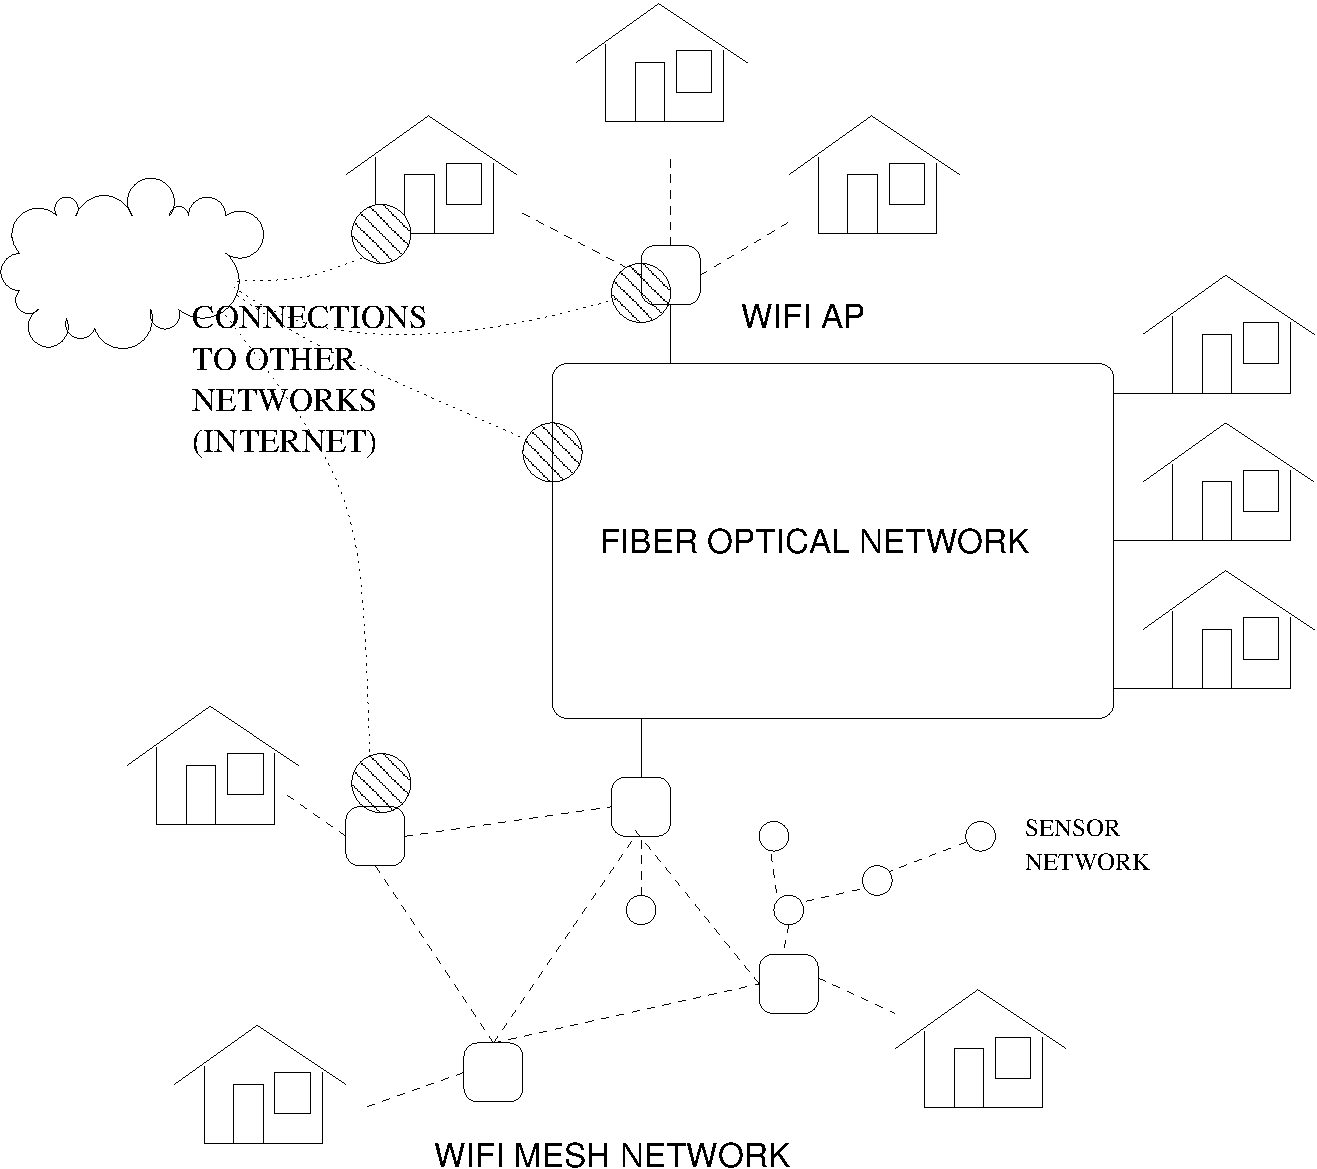
\includegraphics[width=\columnwidth]{figures/hybrid.pdf}
\else
\includegraphics[width=\columnwidth]{figures/hybrid.eps}
\fi
\caption{A hybrid BuB deployment combining different technologies.}
\label{fig:hybrid}
\end{figure}

We have also chosen pilots that can cover multiple cities in Europe.
With the exception of the pilots involving fiber (NQN, FFTx) which by its very nature are localized, the others can be tested and demonstrated in any of the participating cities.

\section{The Open Sensor Network Pilot}
\label{sec:osn}

This pilot is focused on deploying a sensor network which would gather real time data from the environment, such as air quality, noise pollution, etc. This information would be then uploaded to an open data portal to make it publicly available. The ultimate objective of this project is to let developers use this data to build applications that can improve the daily lives of the citizens.

Since this project follows a \emph{BuB} approach each user shall have its own node (or several), which, at the same time would add resources to this network. In case not all nodes aren't connected to the Internet there must be a protocol to interconnect these nodes.

As a power supply there shall be at least two options because each node should have some degree of independency. After all, there is not a predefined environment for these sensors to work on.

For this purpose common wireless protocols such as Wi-Fi, Bluetooth and ZigBee have been compared since this decision will have direct impact on the projectfuture. Although Wi-Fi and Bluetooth have good data rates they are not designed to have a low power consumption which is a key aspect. Also, ZigBee has a low complexity and the best range ---around 550m---, apart from admitting several topologies. Its data rate would be its only drawback, but sensors don't transmit data this often hence Zigbee has been chosen to become the working protocol.

Several sensor board options were available. The university already had Crossbow Telos B nodes which run the TinyOS operating system. This option has many advantages such as built-in multithreading and low-level option tuning. Also, it is open source. Another good choice is Arduino, an open source prototyping system which is commonly used nowadays and has a very large community. Since it is designed with simplicity in mind it lacks the complete set of features that TinyOS can provide, and consequently it is more lightweight, which sinergizes with the project purpose of deploying a battery-powered wireless sensor network.

\section{The Free Europe Wifi Pilot}
\label{sec:few}

The Free Europe WiFi project is based in the original idea that our Italian colleagues are working on. It is called Provincia WiFi, and tries to offer free WiFi internet connection to any Italian citizen. By now it is only available in some regions of that country, so the idea is to extend it to whole Europe. So, our work is to start establishing a similar project in Spain, always having full interoperability with the original project. Thereby, we want to take the next step to extend it to Europe.

In summary, the final idea is: being a European citizen, it is possible to connect to any of the various access point of our network, in order to enjoy of a free internet connection, in every country that participates in the project.

Notice the complexity, not only technical of the project, but also on every European country telecommunication laws. Every region has its own laws in reference of telecommunication organizations, and in the way citizen use the service. From keeping data from the connected users, to meet the rules of the market it's just an example.

This pilot is being carried out by Nacho Justel.

Because of this wide range of different possibilities, it is difficult to create a totally generic prototype, so in order to design it there are many factors to consider.

Talking about the technical aspects of the system, it base its functionality on OpenWISP. OpenWISP (Open Wireless Internet Service Provider) is a software platform that can be used to provide a full, complete WiFi service. It is actually divided into five different modules that will be explained below:

\begin{enumerate}
\item[\fbox{1}] \textbf{OpenWISP User Management System:} 

It is a Ruby on Rails application, that interacts directly with the users. By using this module, the user can get access to the OpenWISP global system to get internet access, password recovery if needed and manage his account.

This module is directly related with third party modules as the FreeRadius server with a MySQL database to sign-up/sign-out and save user information. Once the user is registered in the service, and every time he tries to connect to the network, he will be asked to introduce his username and password to start surfing Internet.

This application has been designed to be integrated with RADIUS authentication solutions.

At this moment, OpenWISP User Management System is being developed to be integrated into FreeRADIUS v2.1, so other implementations are not currently supported.

Some of its features are:
\begin{itemize}
\item User registration via mobile phone, ID card or credit card (Paypal IPN).
\item User interface supporting most common browsers including mobile web browsers.
\item Password recovery via mobile phone or email.
\item Statistics of generated traffic per user.
\item User administration via dedicated admin interface.
\item Admin interface supports role based administration (operator, admin, superadmin).
\item Via admin interface, new users can be added, modified, enabled/disabled or monitoring traffic per user/nationality and logins/registration.
\item English and Italian language translations at the moment.
\end{itemize}

\item[\fbox{2}] \textbf{OpenWISP Geographic Monitoring:}

It is a Ruby on Rails - HTML 5.0 based, web GUI that allows the management staff to get information about the geographic information of the deployed access points. It renders a geographic map of the status your networks: access point up/down/unknown (if an access point has an "unknown" status, then it would not be able to download the configuration to connect to the system from the OpenWISP Access Point Manager. \\

\item[\fbox{3}]\textbf{OpenWISP Captive Portal Manager:}

It is a captive portal written from Scratch with Ruby on Rails. It allows the user surfing the Internet by enabling rules in the server firewall. This module is the operation center of all the system, so all the data that is generated or has as destination the system, will pass through this module. 

Its main features are:
\begin{itemize}
\item Multiple captive portals (one per physical or virtual interface).
\item RADIUS / Local authentication.
\item Experimental traffic shaping per user.
\item Multiple OS support.
\item IPv6 support can be easily implemented.
\end{itemize}


\item[\fbox{4}]\textbf{OpenWISP Access Point Manager:}

It is a Ruby on Rails based web GUI. This module allows the management staff to configure, monitorization and support of deployed access points.\\ It also stores value information about the network, as the amount of traffic each VPN generate, MAC addresses, geographical addresses and network setting, among other data. The access points download the configuration and settings from this module to establish a connection to the gateway.  


\item[\fbox{5}]\textbf{OpenWISP Firmware:}

It is a set of scripts (shell and web cgi) that sits on top of OpenWrt\footnote{OpenWrt is a linux distro for embedded devices that provides a fully writable file structure system with package management. This allows to customize devices keeping freedom from vendor configuration.}. OWF is a no visible module of the system. It is the firmware that every access point has installed to be able to connect to the network. Every time a new access point is connected to the network, it will download the settings from the Access Point Manager, as before explained. If an access point is rebooted without network connectivity, will get no configuration until it could establishes a connection with the OpenWISP Manager, so then, the configuration will be sent to it. 

OpenWISP firmware provides a daemon for retrieving the configuration of some components at the manager:

\begin{itemize}
\item WiFi (currently only for madwifi-ng and ath9k drivers).
\item Networking.
\item Data layer traffic shaping.
\item OpenVPN (data layer, TAP).
\item Unix cron jobs
\end{itemize}

Far from only providing a daemon, it also has a web GUI where:
\begin{itemize}
\item Configuring basic net structure
\item Network parameters.
\item Configuring basic OpenWISP server settings.
\item Performing test and technical fails menu.
\end{itemize}

\end{enumerate}

Also there exists another application based on Ruby/Sinatra that communicates or interacts with the other modules using RESTful services. It is called \textbf{OpenWISP Middleware}.\\This module has different tasks to do depending on the other module that is talking with.

\begin{itemize}

\item By communicating with the OpenWISP Captive Portal Manager, it personalizes the captive page for a group of different access points.\item On the other hand, by interacting with the OpenWISP User Management System, OpenWISP Geographic Monitoring and OpenWISP Access Point Manager, it provides very useful information in a full duplex way.

\end{itemize}

By the moment, we are designing the technical aspects of the spanish implementation of the project, so as soon as we get the design, we will start programming the code to make a first deployment.



\section{The Northern Quarter Network Pilot}
\label{sec:nqn}

This project consists, roughly speaking, on the design, implementation and testing of an optical fiber network in the Northern Quarter (NQ) area of Manchester. This network will provide public free Wi-Fi in that area of the city. The project will be led by the Manchester Digital Development Agency (MDDA), and all the designs and implementations will follow a model they have already developed.


The NQ is home to a wide range of SMEs from many sectors and is a good place for starting businesses to begin their activity and have a trading presence on a centric place of an important city. Providing public WiFi to the NQ will allow businesses to increase their revenues by increasing the number of customers and will give them a way to promote a big range of activities and/or events taking place in the zone. In addition, it is likely that this facts help to support the economy of the NQ area and of the whole city. As mentioned, the NQ area is like a small village in the centre of Manchester where most of the small businesses know each other, and work together to strengthen the economy of the city. This is an important relationship that can be intensified by the implantation of that network, and so the economy will be boosted.



One of the most important aspects of the project, apart from designing and deploying the network, is defining a good pricing model for commercial use. It is a basic point, because it is crucial that the network becomes self-funding and sustainable after the conclusion of the C4EU project. It is, somehow, a critical aspect, and the success of the pilot will strongly depend on the success of the pricing definition. 

\section{FFTx}
\label{sec:fft}

The Rubi pilot consists of the design, implementation, testing and documentation of optical fiber in Rubi, but by some troubles, it has occurred delays in the implementation of fiber in Rubi, therefore without leaving aside this pilot we will realize a project called FFTx. This project will consist to implement the optical fiber under the Bottom-Up Broadband (BuB) model. The FFTx name is because the study includes the main fiber deployments -FFTH/FFTF/FFTP Fiber From The Home/Farm/Premises-. 

To begin the project, we will do a study the BuB model, an investigation of existing fiber types and the advantages that they have over others transmission media. We will do too a comprehensive study on how the optical fiber in Gurb was implemented -Gurb is a municipality where has been successfully implemented the optical fiber under the BuB model-. Finally we will look for the possibility to carry out the implementation of optical fiber under this model in different municipalities (e.g. Rubi).

As you can see, the project has been divided in several tasks, each of them with an aim, but the part that consist of simulating the implementation of the optical fiber in different municipalities it is very important because if we can find the commons to develop and deploy this technology under the BuB model it would be a great contribution to our community.

\section{The Mobile Node Pilot}
\label{sec:mon}

Within this pilot the main idea is to create a free transmission workstation that can be used in the urban space and contributes to the digital mesh through other networks.

The project will consist on creating a mobile wireless workstation that builds or fits in an existent telecommunications 								infrastructure. It will have to be an auto-configurable device and will have the capability to interconnect with a wide range of 					different hardware. Furthermore, it will be able to work in many different spaces and without the need of an ISP.

The project has already started and now it joins to the BuB4EU community in order to be documented and improved if possible.  

\section{Conclusion}
\label{sec:conclusion}

The first BuB4EU pilots to be executed in the framework of the C4EU European project have already been selected.
Each of the students assigned to the pilots have provided a description as well as project charter document.
The students will carefully document their pilots and make this documentation publicly available as a common resource to be shared by the community.




% if have a single appendix:
%\appendix[Proof of the Zonklar Equations]
% or
%\appendix  % for no appendix heading
% do not use \section anymore after \appendix, only \section*
% is possibly needed

% use appendices with more than one appendix
% then use \section to start each appendix
% you must declare a \section before using any
% \subsection or using \label (\appendices by itself
% starts a section numbered zero.)
%


%\appendices
%\section{Proof of the First Zonklar Equation}
%Appendix one text goes here.

% you can choose not to have a title for an appendix
% if you want by leaving the argument blank
%\section{}
%Appendix two text goes here.


% use section* for acknowledgement
\section*{Acknowledgment}

This work has been partially funded by the European Commission (grant CIP-ICT PSP-2011-5).
The views expressed in this technical report are solely those of the authors and do not represent the views of the European Commission.


% Can use something like this to put references on a page
% by themselves when using endfloat and the captionsoff option.
%\ifCLASSOPTIONcaptionsoff
%  \newpage
%\fi



% trigger a \newpage just before the given reference
% number - used to balance the columns on the last page
% adjust value as needed - may need to be readjusted if
% the document is modified later
%\IEEEtriggeratref{8}
% The "triggered" command can be changed if desired:
%\IEEEtriggercmd{\enlargethispage{-5in}}

% references section

% can use a bibliography generated by BibTeX as a .bbl file
% BibTeX documentation can be easily obtained at:
% http://www.ctan.org/tex-archive/biblio/bibtex/contrib/doc/
% The IEEEtran BibTeX style support page is at:
% http://www.michaelshell.org/tex/ieeetran/bibtex/
\bibliographystyle{IEEEtran}
% argument is your BibTeX string definitions and bibliography database(s)
\bibliography{IEEEabrv,my_bib}
%
% <OR> manually copy in the resultant .bbl file
% set second argument of \begin to the number of references
% (used to reserve space for the reference number labels box)
%\begin{thebibliography}{1}

%\bibitem{IEEEhowto:kopka}
%H.~Kopka and P.~W. Daly, \emph{A Guide to \LaTeX}, 3rd~ed.\hskip 1em plus
%  0.5em minus 0.4em\relax Harlow, England: Addison-Wesley, 1999.

%\end{thebibliography}

% biography section
% 
% If you have an EPS/PDF photo (graphicx package needed) extra braces are
% needed around the contents of the optional argument to biography to prevent
% the LaTeX parser from getting confused when it sees the complicated
% \includegraphics command within an optional argument. (You could create
% your own custom macro containing the \includegraphics command to make things
% simpler here.)
%\begin{biography}[{\includegraphics[width=1in,height=1.25in,clip,keepaspectratio]{mshell}}]{Michael Shell}
% or if you just want to reserve a space for a photo:

%\begin{IEEEbiography}{Michael Shell}
%Biography text here.
%\end{IEEEbiography}

% if you will not have a photo at all:
%\begin{IEEEbiographynophoto}{John Doe}
%Biography text here.
%\end{IEEEbiographynophoto}

% insert where needed to balance the two columns on the last page with
% biographies
%\newpage

%\begin{IEEEbiographynophoto}{Jane Doe}
%Biography text here.
%\end{IEEEbiographynophoto}

% You can push biographies down or up by placing
% a \vfill before or after them. The appropriate
% use of \vfill depends on what kind of text is
% on the last page and whether or not the columns
% are being equalized.

%\vfill

% Can be used to pull up biographies so that the bottom of the last one
% is flush with the other column.
%\enlargethispage{-5in}

\appendices

\section{Appendix 1: Free Europe WiFi Project Charter}
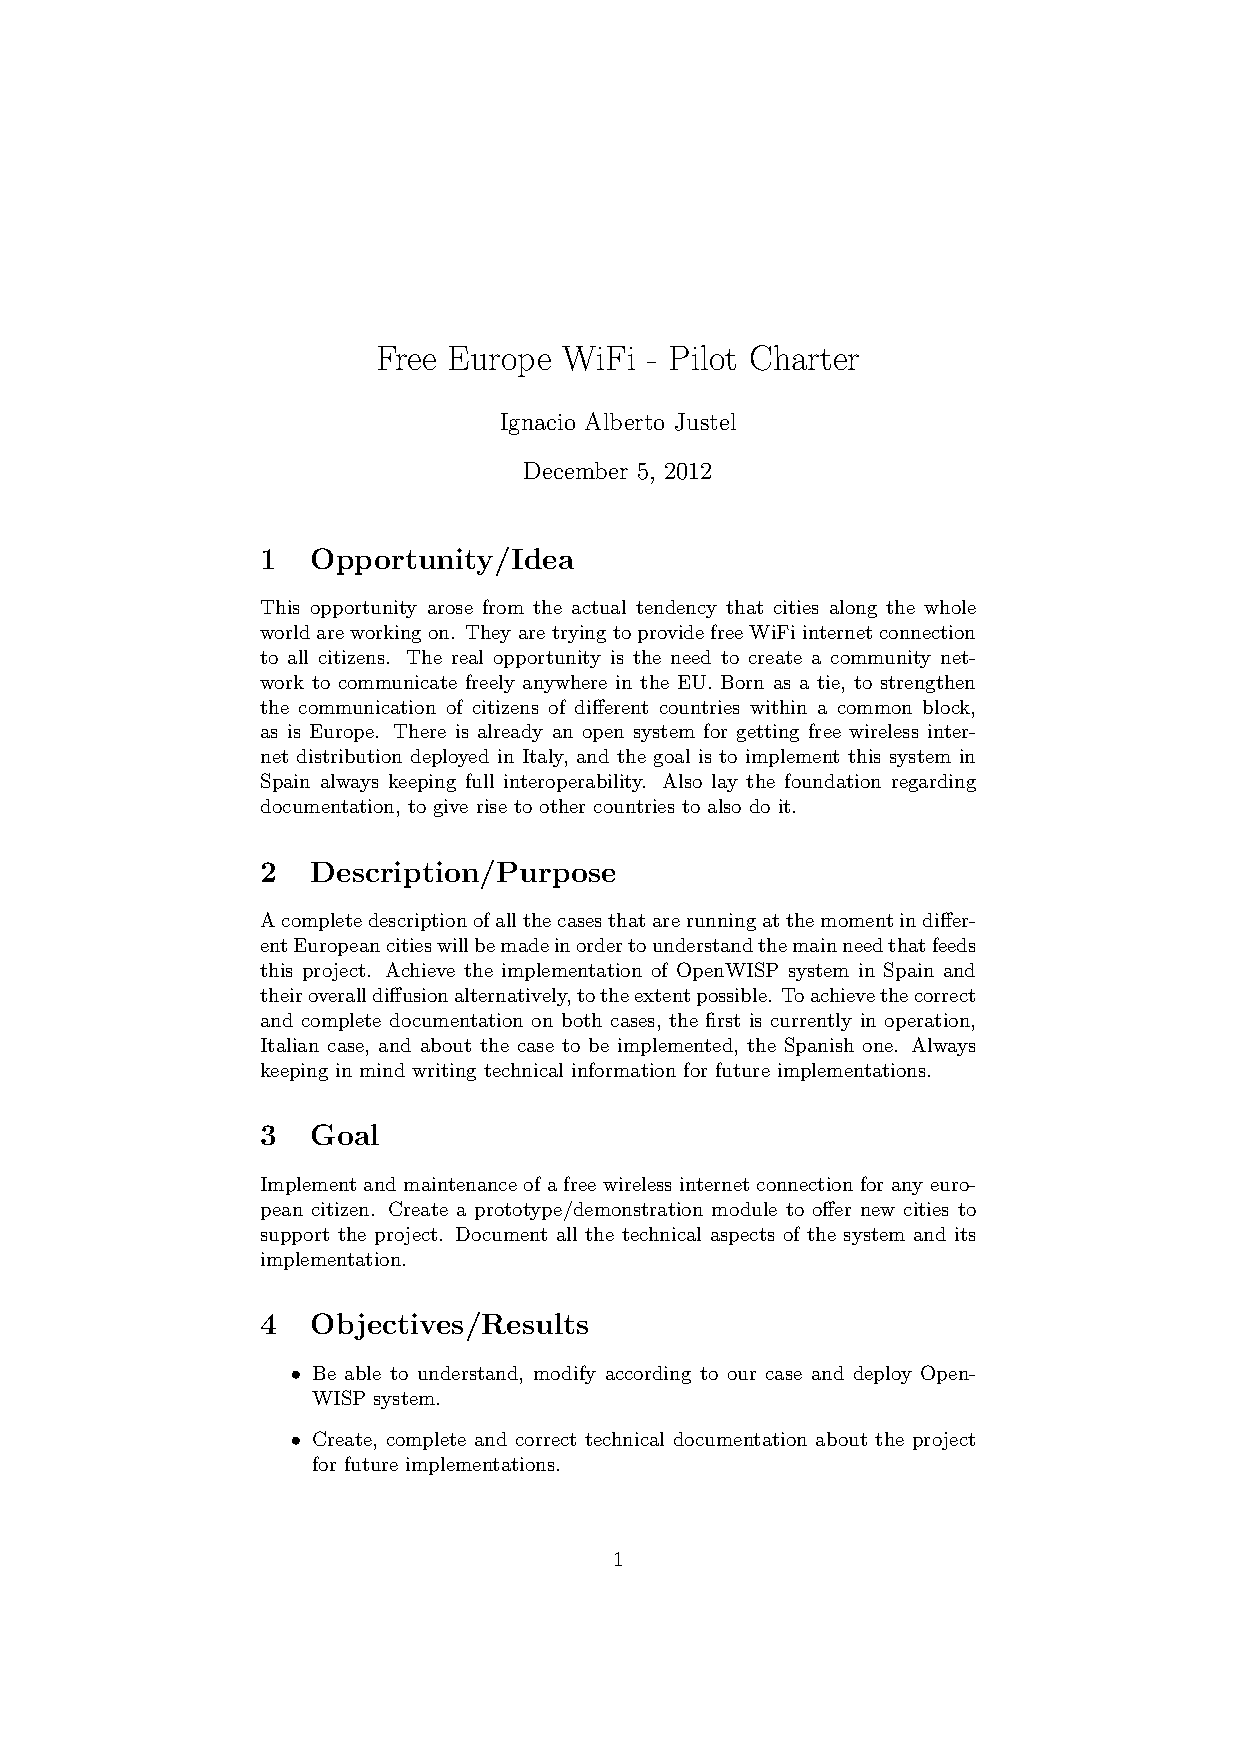
\includepdf[pages={1,2,4}]{projectcharter/projectcharterFEW.pdf}


\section{Appendix 2: FFTx Project Charter}
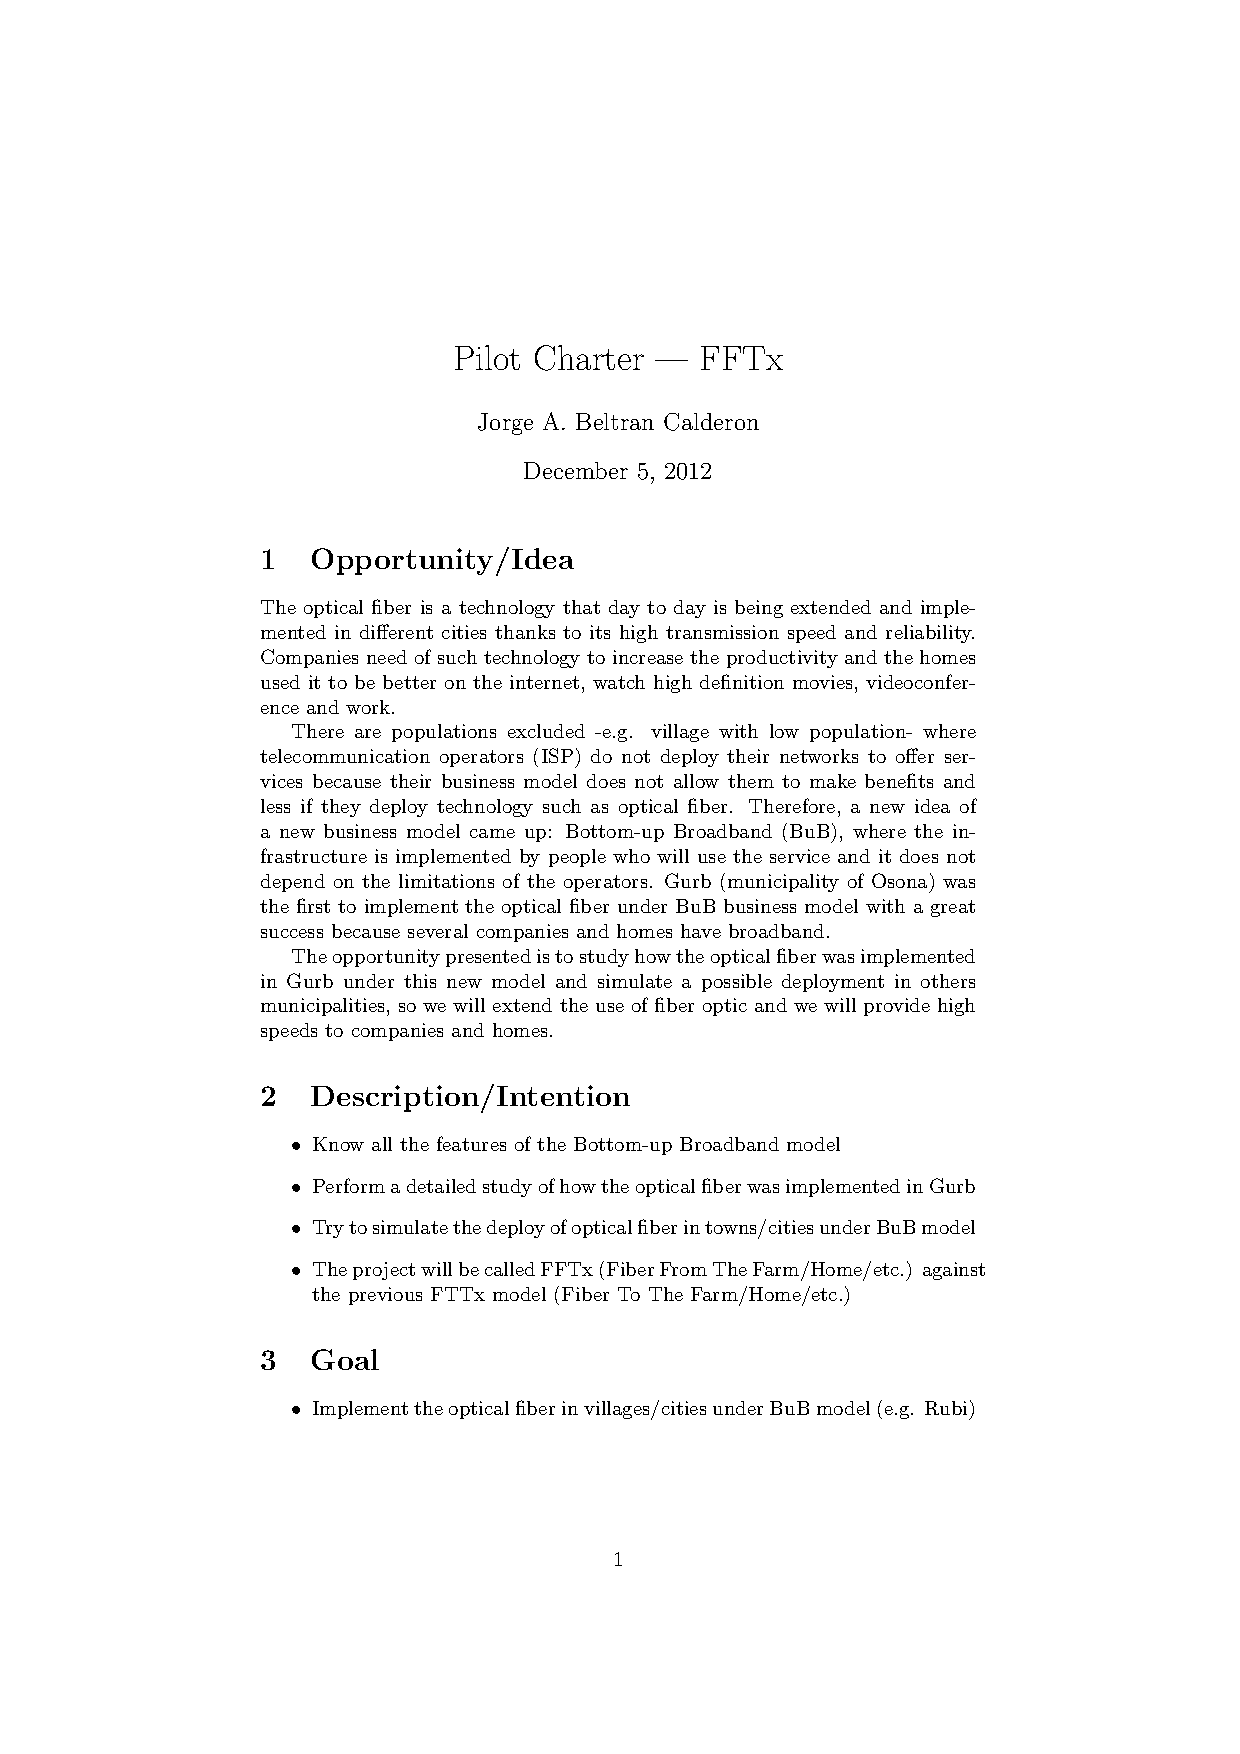
\includepdf[pages={1,2}]{projectcharter/projectcharterFFTx.pdf}

\section{Appendix 3: OSN Project Charter}
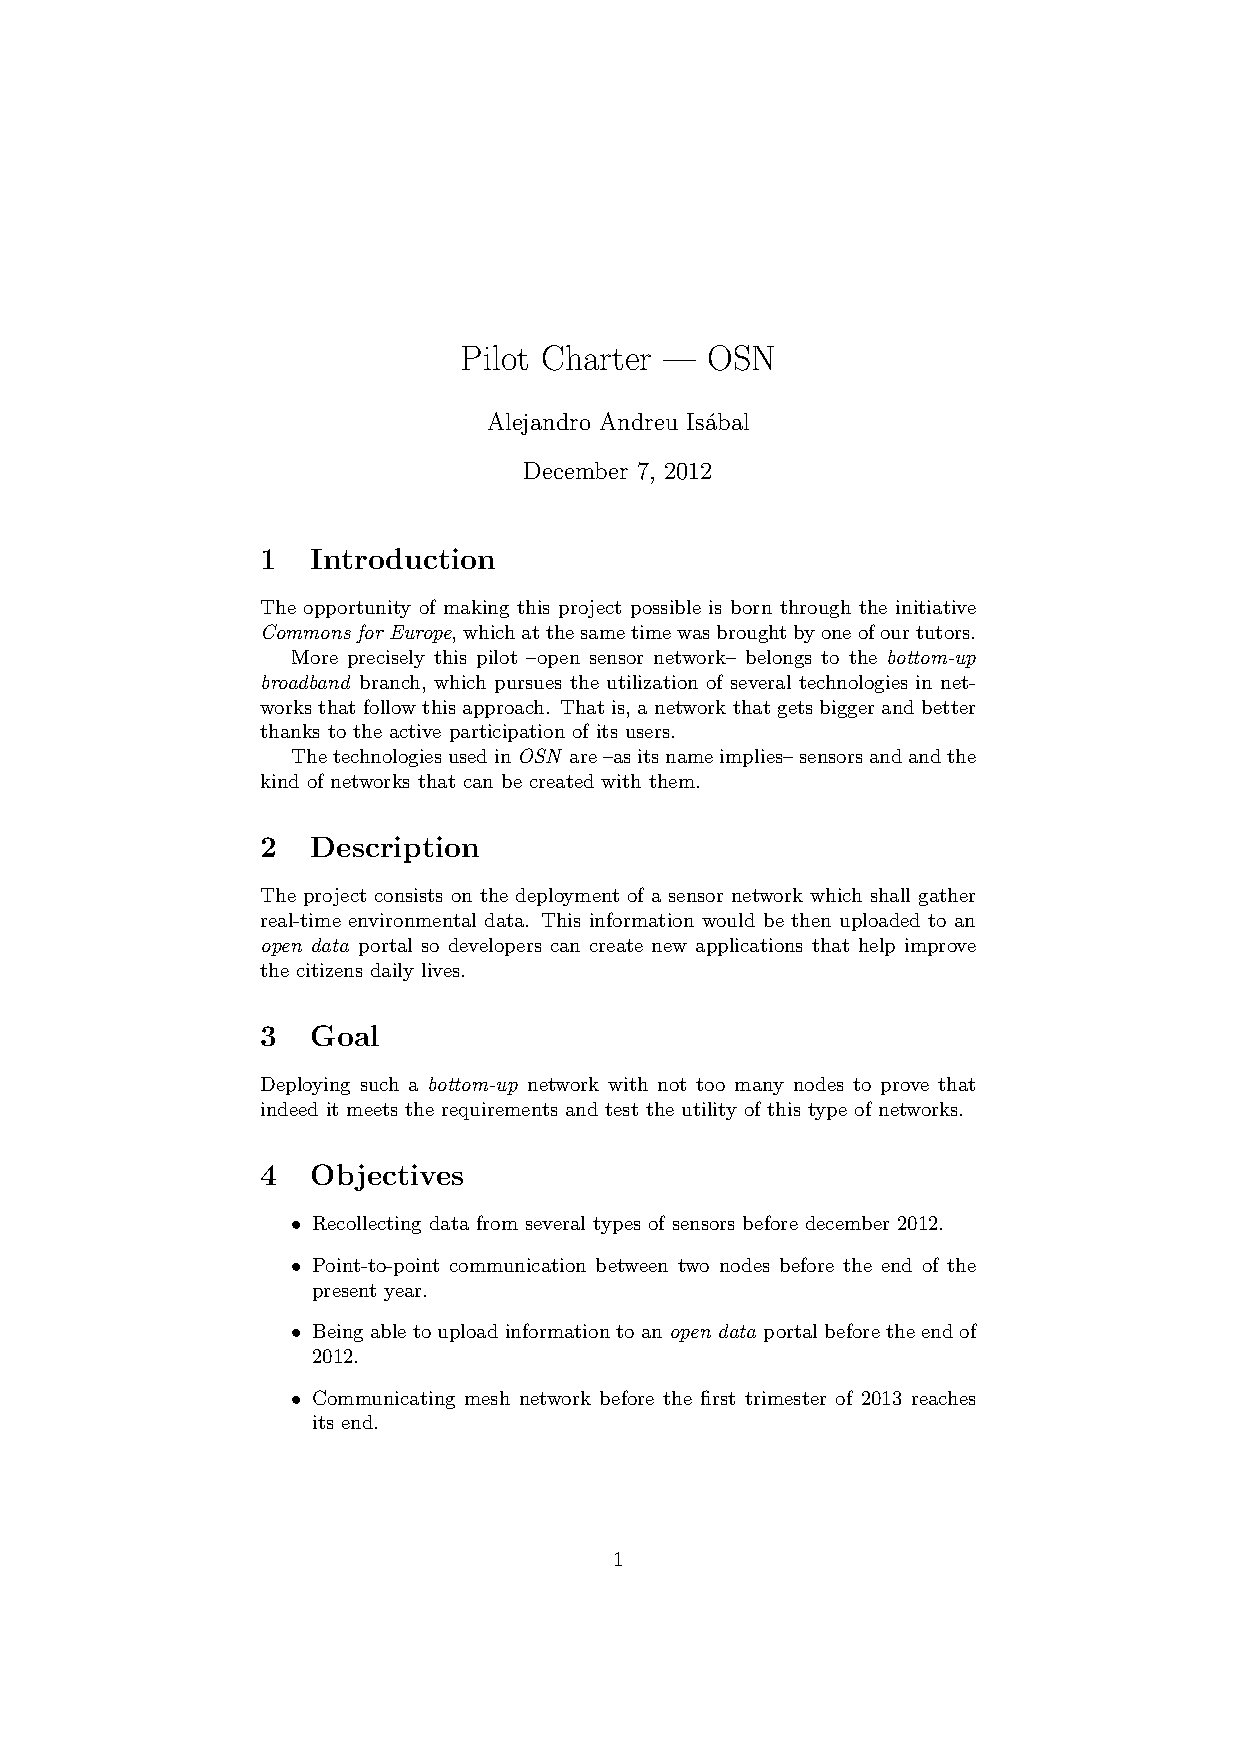
\includepdf[pages={1,2}]{projectcharter/projectcharterOSN.pdf}

% that's all folks
\end{document}


